\documentclass[12pt,oneside,a4paper]{article} % for sharing
\usepackage{apacite}
\usepackage{appendix}
\usepackage{amsmath}
\usepackage{amsthm}
\usepackage{multirow}
\usepackage{amssymb} % for approx greater than
\usepackage{caption}
\usepackage{placeins} % for \FloatBarrier
\usepackage{graphicx}
\usepackage{subcaption}
\usepackage{longtable}
\usepackage{setspace}
\usepackage{booktabs}
\usepackage{tabularx}
\usepackage{xcolor,colortbl}
\usepackage{chngpage}
\usepackage{natbib}
\bibpunct{(}{)}{,}{a}{}{;} 
\usepackage{url}
\usepackage{nth}
\usepackage{authblk}
\usepackage[most]{tcolorbox}
\usepackage[normalem]{ulem}
\usepackage{amsfonts}

% scraped out necessary stuff from hal's loghead file

% new commands defined

%bold faced letters
\newcommand{\bo}[1]{{\bf #1}}

\newcommand{\bm}[1]{\mbox{\boldmath $#1$}}
\newcommand{\kron}{\otimes}
\renewcommand{\vec}{\mbox{vec} \,}

%begin and end equations
\newcommand{\be}{\begin{equation}}
\newcommand{\ee}{\end{equation}}

%begin and end equations without numbers
\newcommand{\bd}{\begin{displaymath}}
\newcommand{\ed}{\end{displaymath}}

%begin and end equation arrays
\newcommand{\bea}{\begin{eqnarray}}
\newcommand{\eea}{\end{eqnarray}}

%begin and end equation arrays without numbers
\newcommand{\beastar}{\begin{eqnarray*}}
\newcommand{\eeastar}{\end{eqnarray*}}

%begin and end matrices
\newcommand{\bmat}[1]{\left(\begin{array}{#1}}
\newcommand{\emat}{\end{array}\right)}

%equation numbers
\newcommand{\enum}[1]{\label{eq:#1}}

%derivatives and elasticities
\newcommand{\der}[2]{{d #1 \over d #2}}
\newcommand{\elas}[2]{{\varepsilon #1 \over \varepsilon #2}}


%partial derivatives and second partial derivatives
\newcommand{\pder}[2]{{\partial #1 \over \partial #2}}
\newcommand{\secpderij}[3]{{\partial^2 #1 \over \partial #2 
            \partial #3}}
\newcommand{\tsecpderij}[3]{\partial^2 #1 / \partial #2 
            \partial #3}  %text second partial

\newcommand{\secpderii}[2]{{\partial^2 #1 \over \partial #2^2}}
\newcommand{\tsecpderii}[2]{\partial^2 #1 / \partial #2^2}
%   text second partial

%matrix transpose symbol
\newcommand{\tr}{{\mbox{\tiny \sf T}}}

%matrix diagonal symbol
%\newcommand{\diag}{\mbox{diag} \,}
\newcommand{\diag}{\mathcal{D}}

\newcommand{\trace}{\mbox{trace}}

\newcommand{\dg}{{\rm{dg}}}

% \mc{number of columns}{position}{item}
\newcommand{\mc}[3]{\multicolumn{#1}{#2}{#3}}
% center a single item in a table
\newcommand{\cent}[1]{\mc{1}{c}{#1}}

\newcommand{\mcal}[1]{\mathcal{#1}}


\newcommand{\str}[1]{\rule{0in}{#1}}
\newcommand{\tbar}[1]{\left. \rule{0in}{#1} \right|}





\newcommand{\rind}{\noindent\hangindent=20pt\hangafter=1}

%%%%%%%%%
% margin adjustments
% these are for US letter size paper; should be adjusted for A4
%%%%%%%%

\textwidth=6.5in
 \oddsidemargin=0in
 %\evensidemargin=0.125in
 %\evensidemargin=0.5in
 \textheight=9.0in
 \topmargin=0.0in
 \headheight=0.0in
 \headsep=0.0in

%%%%%%%%%%%%
% end of margin adjustments
%%%%%%%%%%%% 

%%%%%% stuff from here on not used much %%%%%

% \newtheorem{theorem}{Theorem}[section]
%\newtheorem{theorem}{Theorem}

%\newtheorem{example}{Example}[section]
\newtheorem{example}{Example}

    \newcommand{\exbegin}[1]{\begin{itemize} \item[~]

    \begin{example}{\bf #1} \begin{rm} }
    \newcommand{\exend}{\end{rm}\end{example}
    \end{itemize}}
\newcommand{\scp}[1]{\langle #1 \rangle}
\setcounter{secnumdepth}{3}
\setcounter{tocdepth}{4}

\newtheorem{newfig}{Figure}
\newcommand{\figbegin}{\begin{newfig} \begin{rm} }
\newcommand{\figend}{\end{rm} \end{newfig}}
% commands to change float restrictions
\renewcommand{\topfraction}{0.99}
\renewcommand{\bottomfraction}{0.99}
\renewcommand{\textfraction}{0}
\renewcommand{\floatpagefraction}{0}

\newcommand{\mathbold}[1]{\mbox{\boldmath $\bf#1$}}
% Shultis, Latex Notes, p. 54


%Commands for biblist
\newenvironment{biblist}{\begin{list}{}{\setlength{\leftmargin}{0.15in}% 
\setlength{\itemindent}{-0.15in} \setlength{\parsep}{0.in}%
\setlength{\itemsep}{0.1in}}}{\end{list}} 


% columns for longtable
\newcolumntype{C}[1]{>{\centering\let\newline\\\arraybackslash\hspace{0pt}}m{#1}}
\newcolumntype{L}[1]{>{\raggedright\let\newline\\\arraybackslash\hspace{0pt}}m{#1}}
\usepackage{arydshln} % Dashed lines in matrices


\usepackage[margin=1in]{geometry}
%\doublespacing % for review

% line numbers to make review easier
%\usepackage{lineno}
%\linenumbers

%\usepackage{soul}% for \st{}

%%%%%%%%%%%%%%%%%%%%%%%%%%%%%%%%%%%%%%%%%%%%%%%%%%%%%%%%%%%%%%%%%%%%%%%%%%%%%%
% for section 4 math environments
\theoremstyle{definition}
\newtheorem{definition}{Definition}[section]
\newtheorem{theorem}{Theorem}[section]
\newtheorem{proposition}{Proposition}[section]
\newtheorem{corollary}{Corollary}[proposition]
\newtheorem{remark}{Remark}[section]

%%%%%%%%%%%%%%%%%%%%%%%%%%%%%%%%%%%%%%%%%%%%%%%%%%%%%%%%%%%%%%%%%%%%%%%%%%%%%%

\newcommand\ackn[1]{%
  \begingroup
  \renewcommand\thefootnote{}\footnote{#1}%
  \addtocounter{footnote}{-1}%
  \endgroup
}

% Affiliations in small font size
\renewcommand\Affilfont{\small}

\defcitealias{HMD}{HMD 2016}

% junk for longtable caption
\AtBeginEnvironment{longtable}{\linespread{1}\selectfont}
\setlength{\LTcapwidth}{\linewidth}

% sort van Raalte properly
% #1: sorting key, #2: prefix for citation, #3: prefix for bibliography
\DeclareRobustCommand{\VAN}[3]{#2} % set up for citation

%%%%%%%%%%%%%%%%%%%%%%%%%%%%%%%
\begin{document}


\title{The changing contribution of socioeconomic deprivation to variance in age at death}
%\author{author(s) redacted}
\author[1]{Rosie Seaman\thanks{seaman@demogr.mpg.de}}
\author[1]{Tim Riffe}
\author[2]{Hal Caswell}

\affil[1]{Max Planck Institute for Demographic Research, Rostock, Germany}
\affil[2]{University of Amsterdam}

\maketitle

\begin{abstract}
Mortality inequalities demonstrate a double burden: the most deprived socioeconomic
groups experience the lowest average age of death and the highest variation in age at death. No study has identified how variation in age of death is patterned by area-level socioeconomic deprivation despite the established literature demonstrating that area-level effects are an important part of the explanation for inequalities in risk of death. Two underlying processes drive variation in age at death: individual stochasticity (within-group variance) and heterogeneity (between-group inequality). Limited research has evaluated how these two components have changed over time. We address these research gaps by using population and mortality data for the entire population of Scotland stratified by a validated measure of area-level deprivation that covers the time period 1981-2011.
\end{abstract}

\section{Background}
The association between socioeconomic inequality and mortality is traditionally
evidenced by life expectancy comparisons. The most deprived populations
experience the lowest average age of death, and the least deprived populations
experience the highest. Studies have further demonstrated that the most deprived
populations also demonstrate the highest level of variation in age at death when
measuring socioeconomic inequality by income, education, or occupation \citep{Broennum-Hansen2017,Raalte2011,Sasson2016,Raalte2014}. To our knowledge no study has identified how variation in age
of death is patterned by area-level socioeconomic inequality even though it has long been established that area of residence is
an important part of the explanation for socioeconomic differences in mortality
outcomes \citep{Carstairs1989,Macintyre2002,Tunstall2011}. Area-level measures aim to capture relative deprivation rather than absolute
poverty. Relative deprivation is the idea that not having enough material
cultural or social resources to participate in the accepted way of life in one's
societal context is as important for health as the absolute minimum requirements
for survival \citep{Kearns2000,Carstairs1989,Townsend1987} .
 
Two processes underly variance in age at death: Individual
stochasticity (within-group variance) and heterogeneity (between-group
inequality). Within-group variance arises from differences due to random
demographic processes. The life table assumes that every individual is subject
to the same schedule of mortality rates, such that any
variance in age of death can be interpreted as individual stochasticity. Between-group inequality can arise if individuals at the same age are subject to different mortality rates that may be due to unobserved social, economic or environmental contexts \citep{Hartemink2017}.

One existing study of 11 European countries found that the differences between
educational groups accounted for between 1.2\% and 10.9\% of total variance in
age at death \citep{Raalte2012}. This study used aggregated data for the
years 1990 to 2000, such that time trends could not be assessed. Education may
also be a problematic socioeconomic measure for studying changes in components
over time due to compositional changes \citep{Hendi2015}.  In addition, stratifying data by
education or other acquired states forces the researcher to left-truncate data
at some age, such as 35.
 
We contribute to previous findings by measuring how the within-group and
between-group components of total variance in age at death are patterned by sex
and area-level deprivation over time. We use decennial Census population
estimates and mortality data stratified into population-weighted quintiles
according to a validated area-level measure of relative deprivation. The data
include the whole population of Scotland (ca 5 million persons) and cover the
time period between 1981 and 2011. Using population-weighted quintiles according
to an area-level measure of deprivation has two advantages. Firstly, it is applicable to the entire population meaning that age truncation is not necessary. Secondly, it is a relative measure of deprivation, meaning that there is always a notional 20\% most deprived compared to a notional 20\% least deprived even though absolute levels of deprivation may have changed over time.



\section{Data and methods}

\subsection{Area level deprivation}
Census population estimates and mortality data\footnote{Mortality data used
came from 1980-1982, 1990-1991, 2000-2002 and 2010-2012 to increase the
number of events centered around each census. 1990-1991 is just a two-year
numerator sample due to geographical boundary changes occurring in 1990.
Corresponding Census population estimates are adjusted accordingly.} by single
year of age and sex for each part-postcode (zip code) sector in Scotland were obtained via a commissioned request to National Records of Scotland. There are around 1,012 part-postcode sectors in Scotland at each Census year each with an average population size of 5,000 individuals.
 
Population-weighted quintiles (each 20\% of the population) were created by
aggregating the 1,012 part-postcode sectors according to Carstairs score of
deprivation. The Carstairs score is a z-score for each part-postcode sector
that is derived from four individual-level census variables: overcrowding, male
unemployment, low social class, and no car ownership. The Carstairs Score
(z-score) reflects the material resources that provide the means to access the
goods, services, amenities, and physical environment seen as expected
in society \citep{Carstairs1989}. This means the Carstairs score is a method of capturing relative deprivation at the contextual level.

Deaths and census population denominators were used to construct complete
lifetables for each deprivation quintile, at each Census year, for males and
females seperately (40 lifetables in total). The Human Mortality Database
protocol was used to extrapolate age specific mortality rates from ages 85 to
110 \citep{Wilmoth2007}.\footnote{Specifically, we apply equations (53) and
(54) from the HMD protocol v5, modified to use information from ages 75+
rather than 80+.} From the complete lifetables we compute remaining
life expectancy and the conditional standard deviation of the remaining lifespan
distribution. Lifetable standard deviations are a common measure of the
variability applied to the distribution of age at death \citep{Raalte2013}. Details of the within-group and between-group component calculations are given in the following subsection.


\subsection{Variance decomposition}
Lifetable variance is calculated and decomposed into within- and between-group
components using Markov chain methods \citep{Caswell2001}\citep{Caswell2009}\citep{Caswell2014}. From the lifetable, we extract
conditional single-age death probabilities, $q_x$, and take its complement,
$p_x$. We then calculate the survival matrix for the $i^{th}$
quintile, $\bo U_i$ as:
\begin{equation}
\bo U_i = 
\begin{bmatrix}
    0     & \hdots  & \hdots &  \hdots  & 0 \\
    p_{1} &   &    &    &  \vdots \\
    0 & \ddots &   &   & \vdots \\
    \vdots & & \ddots & & 0\\
   0 &  \hdots & 0 & p_{\omega-1}  & p_{\omega}
\end{bmatrix}
\end{equation}
Conditional remaining survivorship is calculated as:
\begin{equation}
\mathbf{N}_i = (\mathbf{I} - \mathbf{U}_i )^{-1} \quad .
\end{equation}
$\mathbf{N}_i$ ends up being 0s in the upper triangle, and conditional remaining
survivorship in columns descending from the subdiagonal. The moments of longevity for individuals in group $i$ are $\bm \eta_1^{(i)}$ and $\bm \eta_2^{(i)}$. 
\begin{equation}
\bm \eta_1^{(i)} = (1^\tr \bm N_i)^\tr
\end{equation}
The second moment is defined as:
\begin{equation}
\bm \eta_2^{(i)} = \left[ 1^\tr \bm N_i (2 \bm N_i - \bm I)\right]^\tr
\end{equation}
The vectors with the means and variances, for group $i$, are
\bea
E(\bm \eta^{(i)}) &=& \bm \eta_1^{(i)} \\
V(\bm \eta^{(i)}) &=& \bm \eta_2^{(i)} - \left[ \bm \eta_1^{(i)} \ \circ \bm \eta_1^{(i)} \right]
\eea

To carry out calculations we procede by creating vectors that contain the
combined age and stage specific values
\bea
E(\tilde{\bm \eta}) = \bmat{c}
E(\bm \eta^{(1)}) \\
\vdots\\
E(\bm \eta^{(g)})
\emat
\eea
and a similar vector for variances $V(\tilde{\bm \eta})$. The tilde indicates
that these combine both age and quintile values, with length = $g \omega$.

The next step is to calculate the means and variances of remaining longevity, at
each age $x$, within each group, as follows.
\bea
E(\bm \eta(x)) &=& \left( \bo I_g \kron \bo e_x^\tr \right) E(\tilde{\bm \eta}) \qquad x=1,\ldots,\omega  \\[1ex]
V(\bm \eta(x)) &=& \left( \bo I_g \kron \bo e_x^\tr \right) V(\tilde{\bm \eta}) \qquad x=1,\ldots,\omega
\eea
where $\bo e_x$ is a vector of length $\omega$ with a 1 in the $x$th position and zeros elsewhere. The resulting vectors here are of dimension $g \times 1$.

At age $x$ the cohort consists of a mixture of the $g$ different groups ($g=5$
for quintiles, 10 for deciles) with mixing distribution
$\bm \pi(x)$ generated by the differential survival of groups within the cohort.
Since we are not modelling transitions of individuals among deprivation
quintiles, the mixing distribution at age $x$ is simply given by
\be
\pi_i(x) = \bm 1^\tr \left( \bo U_i^x \bo e_1 \right) /5\qquad i=1,\ldots, 5
\ee
where $\bo e_1$ is a vector with a 1 in the first entry and zeros elsewhere.
This mixture assumes a stationary mixture of subpopulations. Raw weighting is also possible, and gives similar results.

At age $x$ remaining life expectancy for the total population is
\bea
E (\eta_x) &=& E_{\bm \pi(x)} \left[ E(\bm \eta(x)) \right] \\[1ex]
&=& \bm \pi(x)^\tr E(\bm \eta(x)) \\[1ex]
&=& \left( \bm \pi(x)^\tr \kron \bo e_x \right) E(\tilde{\bm \eta}) \qquad x=1,\ldots,\omega
\eea
Notice that $\eta_x$ is a scalar. The remaining life expectancy at age $x$ is a
simple average weighted by the mixing distribution.

The variance in $\eta_x$ is
\be
V(\eta_x) = V_{\rm within} + V_{\rm between}
\ee
with
\bea 
V_{\rm within} &=& E_{\bm \pi(x)} \left[ \str{2.5ex}V \left( \bm \eta(x) \right) \right]  \\[1ex]
&=&
\bm \pi(x)^\tr V(\bm \eta(x) )\\[1ex]
&=& \left( \bm \pi(x)^\tr \kron \bo e_x^\tr \right) V(\tilde{\bm \eta}(x)) 
\eea
and
\bea
V_{\rm between} &=& V_{\bm \pi(x)} \left[ \str{2.5ex} E \left( \bm \eta(x) \right) \right] \\
&=&
\bm \pi(x)^\tr \left[ \str{2.5ex} E(\bm \eta(x) ) \circ E(\bm \eta(x) ) \right] - 
\left[ \str{2.5ex} \bm \pi(x)^\tr E(\bm \eta(x) \right]^2
\eea
Again, $V(\eta_x)$ is a scalar.

\section{Preliminary results}
% You can do automatic table and fig referencing like this:
Table~\ref{tab:LESD0m} and Table~\ref{tab:LESD0f} show the life expectancy and
variation in age at death for males and females, respectively, in each
deprivation quintile at each Census year. The same tables reporting life expectancy and variation in age at death conditional upon survival to age 35 are included in the appendices.

% Table generated by Excel2LaTeX from sheet 'Sheet1'
\begin{table}[htbp]
  \centering
  \caption{Life expectancy and standard deviation for males, age 0.}
  \label{tab:LESD0m} % add this to give a label
    \begin{tabular}{lrrrrrrrr}
          & \multicolumn{2}{c}{1981} & \multicolumn{2}{c}{1991} & \multicolumn{2}{c}{2001} & \multicolumn{2}{c}{2011} \\
    \midrule
    quintile & \multicolumn{1}{c}{ex} & \multicolumn{1}{c}{sd} & \multicolumn{1}{c}{ex} & \multicolumn{1}{c}{sd} & \multicolumn{1}{c}{ex} & \multicolumn{1}{c}{sd} & \multicolumn{1}{c}{ex} & \multicolumn{1}{c}{sd} \\
    \midrule
    1 (least dep.) & 71.6  & 15.4  & 74.5  & 14.4  & 77.6  & 13.7  & 80.2  & 13.6 \\
    2     & 69.9  & 16.1  & 72.9  & 14.9  & 75.3  & 15.1  & 78.5  & 14.6 \\
    3     & 69.1  & 16.2  & 72.1  & 15.4  & 73.9  & 15.4  & 77.0  & 15.1 \\
    4     & 68.2  & 16.2  & 70.4  & 16.1  & 72.2  & 16.1  & 75.3  & 15.6 \\
    5 (most dep.) & 66.4  & 16.4  & 68.3  & 16.5  & 69.0  & 17.2  & 72.4  & 16.5 \\
    Total pop. & 69.0  & 16.1  & 71.6  & 15.6  & 73.5  & 15.8  & 76.7  & 15.4 \\
    \bottomrule
    \end{tabular}%
  \label{tab:addlabel}%
\end{table}%


% Table generated by Excel2LaTeX from sheet 'Sheet1'
\begin{table}[htbp]
  \centering
  \caption{Life expectancy and standard deviation for females, age 0.}
   \label{tab:LESD0f}
    \begin{tabular}{lrrrrrrrr}
          & \multicolumn{2}{c}{1981} & \multicolumn{2}{c}{1991} & \multicolumn{2}{c}{2001} & \multicolumn{2}{c}{2011} \\
    \midrule
    quintile & \multicolumn{1}{c}{ex} & \multicolumn{1}{c}{sd} & \multicolumn{1}{c}{ex} & \multicolumn{1}{c}{sd} & \multicolumn{1}{c}{ex} & \multicolumn{1}{c}{sd} & \multicolumn{1}{c}{ex} & \multicolumn{1}{c}{sd} \\
    \midrule
    1 (least dep.) & 77.1  & 14.9  & 79.1  & 14.1  & 81.3  & 13.0  & 83.4  & 12.8 \\
    2     & 75.8  & 15.3  & 78.6  & 13.9  & 80.4  & 13.6  & 82.1  & 13.5 \\
    3     & 75.1  & 15.6  & 77.7  & 14.7  & 78.9  & 14.5  & 80.9  & 13.9 \\
    4     & 74.4  & 15.7  & 76.6  & 14.8  & 78.1  & 14.6  & 80.0  & 14.0 \\
    5 (most dep.) & 72.8  & 16.3  & 74.9  & 15.9  & 76.3  & 15.7  & 77.9  & 15.1 \\
    Total pop. & 75.0  & 15.6  & 77.3  & 14.8  & 78.9  & 14.4  & 80.9  & 14.0 \\
    \bottomrule
    \end{tabular}%
  \label{tab:addlabel}%
\end{table}%

The most deprived quintile experiences the lowest life expectancy and
the highest variation in age at death (highest standard deviation) at each year. For males there was an
increase in variation in age at death between 1991 and 2001. Although there was
some improvement between 2001 and 2011, variation in age at death was very
similar to the level experienced 30 years earlier. Females from the most
deprived quintile have experienced decreasing variation in age at death (decreasing standard deviation) but the
decrease was greater for the least deprived. The change in standard
deviation over time, across all ages is sown in Figure ~\ref{fig:sdtotal}. Male
total variation has increased somewhat, and female total variation has changed
very little over the time period studied.

Figure~\ref{fig:decompbtwn} shows the proportion of the total difference in
variation in age at death that is due to differences between area level deprivation. For males and females the proportion of variation explained by between group inequality has increased over time. The increase in this component was greater in magnitude for males than for females.

\begin{figure*}[t!]
    \centering
      \caption{Standard deviation of remaining lifespan for total population by age, Census years
      1981 until 2011.}
      \label{fig:sdtotal}
    \begin{subfigure}[t]{0.5\textwidth}
        \centering
        \caption{Males}
        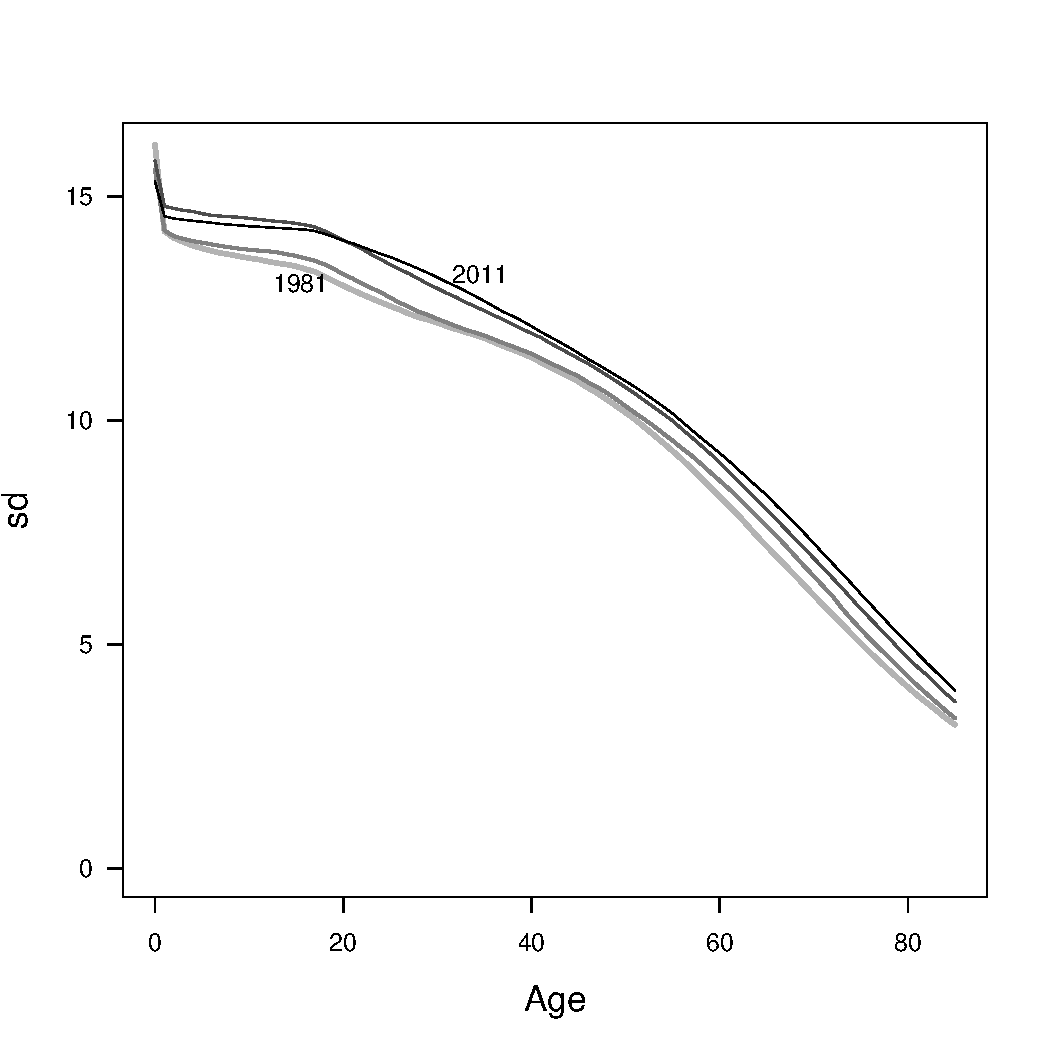
\includegraphics[width=\textwidth]{Figures/TotalsdMales.pdf}
    \end{subfigure}%
    ~ 
    \begin{subfigure}[t]{0.5\textwidth}
        \centering
        \caption{Females}
        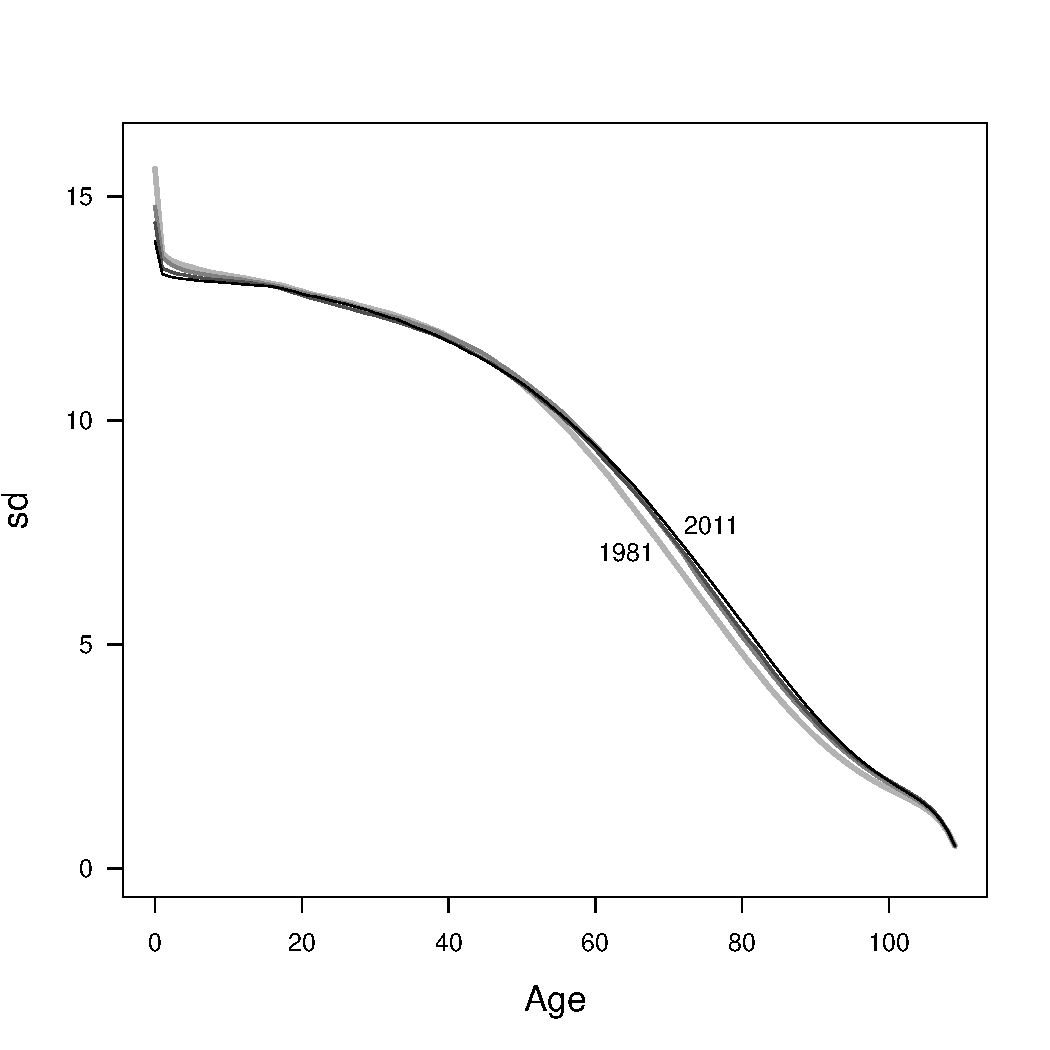
\includegraphics[width=\textwidth]{Figures/TotalsdFemales.pdf}
    \end{subfigure}
\end{figure*}

\begin{figure*}[t!]
    \centering
      \caption{Proportion of variance due to differences between deprivation
      quintiles by age, Census years 1981 until 2011.}
      \label{fig:decompbtwn}
    \begin{subfigure}[t]{0.5\textwidth}
        \centering
        \caption{Males}
        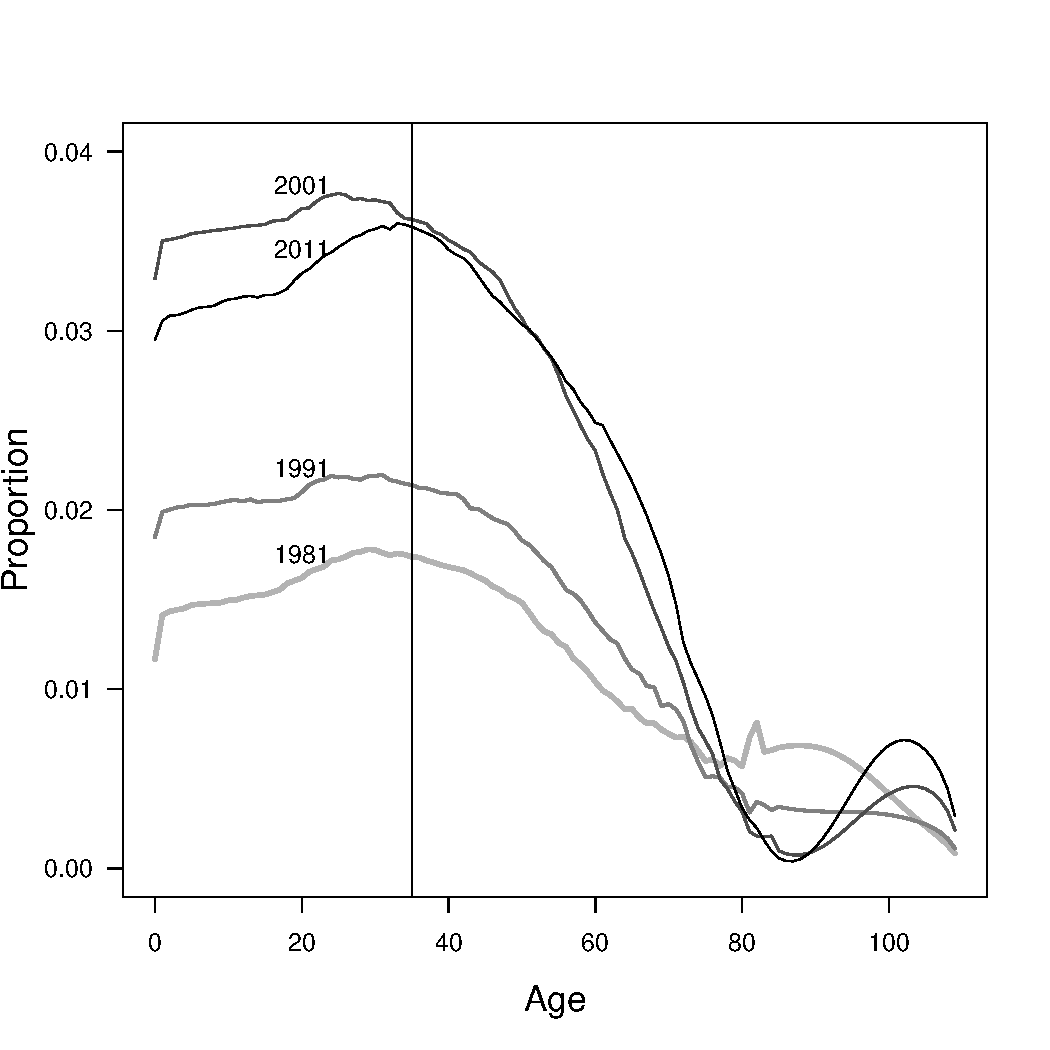
\includegraphics[width=\textwidth]{Figures/BetweenPropMales.pdf}
    \end{subfigure}%
    ~ 
    \begin{subfigure}[t]{0.5\textwidth}
        \centering
        \caption{Females}
        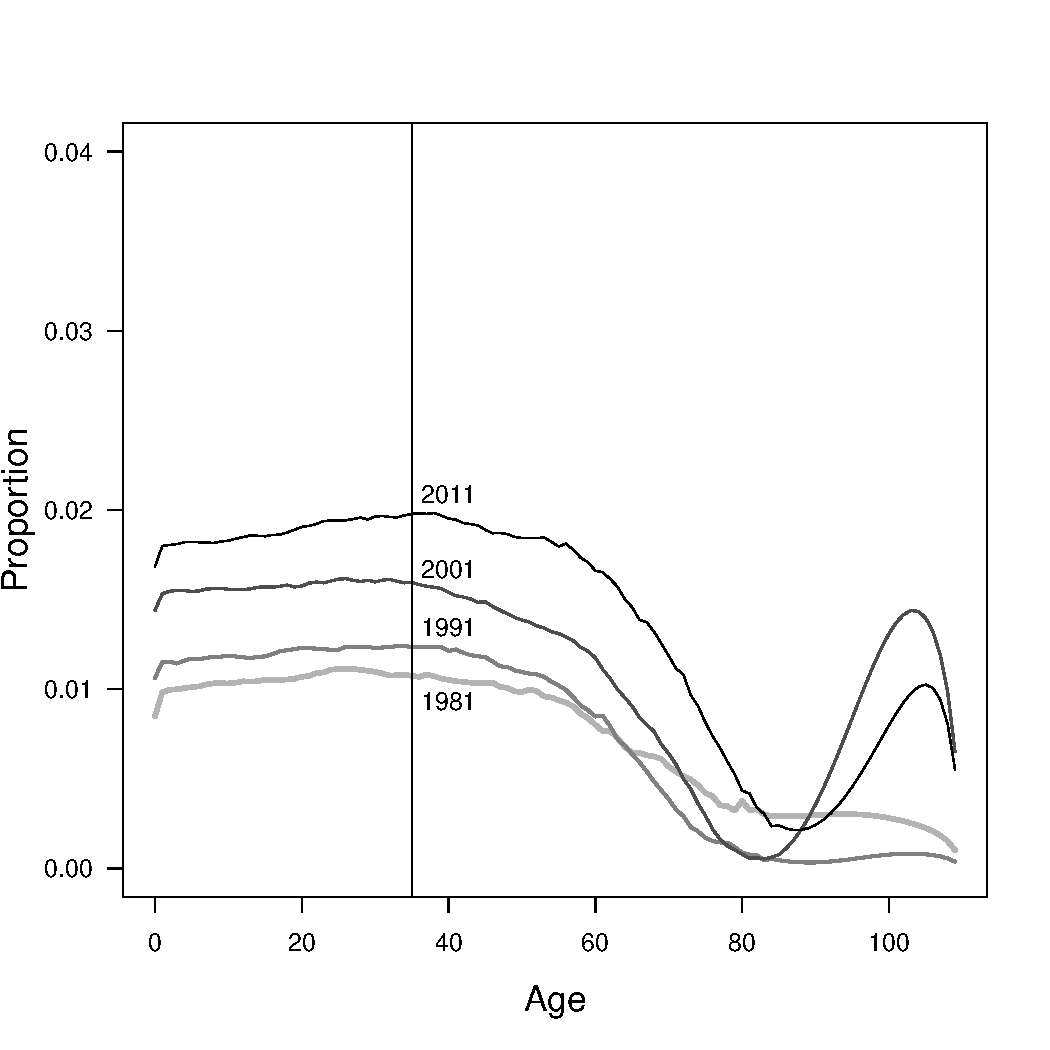
\includegraphics[width=\textwidth]{Figures/BetweenPropFemales.pdf}
    \end{subfigure}
\end{figure*}

\FloatBarrier
\subsection{Sensitivity analysis}
We tested the sensitivity of our results to the size of deprivation group by
replicating the analysis using deciles of deprivation, each representing 10\% of
the population. The conclusions were the same for males and for females.
However, the increase in the between group component over time was greater in
magnitude when using deciles. We chose to report results for quintiles of
deprivation as they are the preferred analytical grouping for routine reporting
of health measures in Scotland \citep{Health2017}.

\section{Discussion and conclusion}

\subsection{Summary of main findings}
Deprivation differences in age at death were evident at all Census years when measuring socioeconomic inequality by area-level. Those living in the most deprived areas can expect to live the shortest lives and experience the greatest variation in age at death: a double burden of mortality inequality. The difference between deprivation groups was larger for males than for females. Males from the most deprived quintile experienced increasing variation in age at death between 1991 and 2001 so that the level of variation in 2011 was the same as that experienced 30 years earlier. The between group component of inequality also increased over the time period.

\subsection{Strengths and limitations}
The data used for this study includes the most robust population estimates and mortality data for the entire population of Scotland. Using a validated area-level measure of socioeconomic inequality meant that complete lifetables could be constructed and no ages were truncated from the analysis. However, it is important to acknowledge the reasons why studies interested in the social distribution mechanisms of adult mortality may consider restricting analysis to older ages. \citet{Smits2009} suggest only looking at ages 15+ because these are the ages where 80\% of deaths in developed countries now occur. Looking only at adult mortality may better reflect the causes of death driving mortality change in more recent time periods: infectious disease and effective medical intervention historically reduced infant and childhood deaths rapidly but reductions in adult mortality are influenced by more complex mechanisms that change slowly \citep{Smits2009,Vallin2004}. Our results indicate that the age at which the difference in variation in age at death is greatest is around 35 years old. This provides some reassurance for studies that are forced to truncate out younger age groups: the peak of variation in age at death (at least in developed countries) is likely to be captured. 

We recognize that our results are vulnerable to the ecological fallacy : it is possible that the association found at the area-level may differ from the association found at the individual \citep{Diez2002}. The consistency of our findings with the existing literature on socioeconomic inequalities in variation in age at death \citep{Broennum-Hansen2017,Raalte2014} indicates that the findings by area-level deprivation are not an artefact. This does not mean that area-level measures and individual level measures are substitutes for one another. Area-level measures ‘capture characteristics of populations’ and individual level measures ‘capture characteristics of individuals’ \citep{Leyland2007}. An example helps to illustrate the contentions. GPs aiming to reduce inequalities between individuals by providing preventative screening programmes may rely on area-level indicators to target those who are most deprived but may target an individual in a deprived area who is actually well-off. So relying on an area-level measure to reduce health inequalities between individuals can be problematic if there is an assumption that the underlying characteristics of the population are socially homogenous \citep{Fischbacher2014}. We acknowledge that deprived individuals do not exclusively reside in deprived areas and affluent individuals do not exclusively reside in affluent areas \citep{Leyland2007}.

The Carstairs score has been the focus of further criticisms. For example, the meaning of car ownership is fundamentally different for individuals in rural contexts compared to urban contexts. It is also acknowledged that overcrowding may occur out of choice and for cultural reasons rather than simply being a marker of deprivation \citep{Fischbacher2014}. Therefore it has been suggested that the Carstairs score may be an out of date measure of socioeconomic deprivation \citep{Schofield2016,Tunstall2011} because the relevance of the variables used for capturing the meaning of deprivation varies across contexts and over time \citep{Norman2010}. In response, it was demonstrated that the scores for each postcode sector at each Census year are highly correlated despite changes to the formal definitions of the variables. This is interpreted as evidence that the underlying information the variables aim to capture is similar or that deprivation has remained stable over time \citep{Leyland2007}.

\section{Conclusion}
Area-level measures of deprivation are an invaluable tool for population health research. Perhaps more importantly, they have pragmatic advantages for governments seeking to identify how resources should be distributed across societies and are actively used by policies which intervene on neighborhoods or communities rather than individuals \citep{Allik2016, Roux2001,Robert1999,TheScottishGovernment2016}. For these reasons, it is important that more countries evaluate inequalities in variation in age at death by an area-level measure of socioeconomic inequality. This will help to identify if increasing contributions from between group inequality to total variation in age at death is a finding that is dependent upon, and thus amenable to, country specific contexts.  


\bibliographystyle{apalike}
\bibliography{references}


\section{Appendices}
% Table generated by Excel2LaTeX from sheet 'Sheet1'
\begin{table}[htbp]
  \centering
  \caption{Life expectancy and standard deviation for males, age 35.}
    \begin{tabular}{lrrrrrrrr}
          & \multicolumn{2}{c}{1981} & \multicolumn{2}{c}{1991} & \multicolumn{2}{c}{2001} & \multicolumn{2}{c}{2011} \\
    \midrule
    quintile & \multicolumn{1}{c}{ex} & \multicolumn{1}{c}{sd} & \multicolumn{1}{c}{ex} & \multicolumn{1}{c}{sd} & \multicolumn{1}{c}{ex} & \multicolumn{1}{c}{sd} & \multicolumn{1}{c}{ex} & \multicolumn{1}{c}{sd} \\
    \midrule
    1 (least dep.) & 38.4  & 11.4  & 40.9  & 11.2  & 43.7  & 11.3  & 46.3  & 11.1 \\
    2     & 37.1  & 11.6  & 39.5  & 11.6  & 41.9  & 11.8  & 44.7  & 12.0 \\
    3     & 36.4  & 11.8  & 38.8  & 11.8  & 40.5  & 12.2  & 43.4  & 12.4 \\
    4     & 35.5  & 11.8  & 37.6  & 11.9  & 39.1  & 12.5  & 41.7  & 13.0 \\
    5 (most dep.) & 33.8  & 12.1  & 35.8  & 12.3  & 36.6  & 13.2  & 39.2  & 13.5 \\
    Total pop. & 36.2  & 11.8  & 38.5  & 11.8  & 40.3  & 12.4  & 43.1  & 12.6 \\
    \bottomrule
    \end{tabular}%
  \label{tab:addlabel}%
\end{table}%


% Table generated by Excel2LaTeX from sheet 'Sheet1'
\begin{table}[htbp]
  \centering
  \caption{Life expectancy and standard deviation for females, age 35.}
    \begin{tabular}{lrrrrrrrr}
          & \multicolumn{2}{c}{1981} & \multicolumn{2}{c}{1991} & \multicolumn{2}{c}{2001} & \multicolumn{2}{c}{2011} \\
    \midrule
    quintile & \multicolumn{1}{c}{ex} & \multicolumn{1}{c}{sd} & \multicolumn{1}{c}{ex} & \multicolumn{1}{c}{sd} & \multicolumn{1}{c}{ex} & \multicolumn{1}{c}{sd} & \multicolumn{1}{c}{ex} & \multicolumn{1}{c}{sd} \\
    \midrule
    1 (least dep.) & 43.4  & 11.7  & 45.1  & 11.5  & 47.0  & 11.1  & 49.0  & 49.0 \\
    2     & 42.2  & 12.0  & 44.4  & 11.7  & 46.1  & 11.5  & 47.9  & 47.9 \\
    3     & 41.6  & 12.2  & 43.8  & 12.1  & 45.0  & 12.0  & 46.7  & 46.7 \\
    4     & 41.0  & 12.1  & 42.7  & 12.3  & 44.1  & 12.2  & 45.7  & 45.7 \\
    5 (most dep.) & 39.6  & 12.7  & 41.4  & 12.8  & 42.6  & 13.1  & 43.9  & 43.9 \\
    Total pop. & 41.5  & 12.2  & 43.4  & 12.2  & 44.9  & 12.1  & 46.7  & 46.7 \\
    \bottomrule
    \end{tabular}%
  \label{tab:addlabel}%
\end{table}%


\end{document}